\section{\tool}
\label{sec:badusb}
\subsection{Threat Model}
We build our threat model on the basic assumptions that common users without technical background would not treat normal-looking USB device as highly dangerous and be cautious about them. These assumptions are approved in a relevant work about charging attack\cite{JFCImpact}. Moreover, we neglect the effect of notification about common USB device, as normal users usually are not equipped with the necessary knowledge to fully understand such notices. In fact, during our experiment, no device had security notifications raised about suspicious USB devices and only mobile devices had raised charging notification about our \tool, which is not a sufficient warning towards users.

We also assume the victim's device is equipped with fully functional USB 3.x protocol and USB Type C connector. As the USB 3.x standard is more and more common nowadays, this assumption can be easily fulfilled especially in recent devices.
\subsection{Motivation}
\noindent\outline{Limitation of Rubber Ducky}\\
\outline{Our functionality different mode listing?}\\
\hongyi{The following mode is to be further decided}
\outline{Automatic Scripting Mode}\\
\outline{Remote Control Mode}\\
\outline{OCR/QR Recognition Mode}\\
As we introduced in the Section~\ref{sec:related_work}, there are plenty of existing work \shuqing{Add citation} focusing on BadUSB attack. 
Many of these take advantage of the \textit{trust-by-default} policy of PC, pretend to be normal HID devices and utilize USB protocol to perform attacks. 
However, these attacks suffer from various drawbacks:
\ding{182} attackers can only simulate limited types of devices such as HIDs (like keyboards and mice) and disks, which makes the attacks less effective;
\ding{183} accurate attacks couldn't be performed due to lack of user interface (UI).
Whatever HID the attackers simulate their USB devices to be, they couldn't obtain the UI to check the current situation, which makes it nearly impossible to carry out their attacks precisely or confirm the effects after attacks.

In this work, we utilized the new features of USB 3.x \cite{usb31} \cite{usb32} to address the problems above.
Benefiting from latest protocol, we simulated external display and thus obtained the video stream to perform accurate attacks.

\subsection{Implementation}
\noindent\hongyi{The following mode is to be further decided}\\
\outline{DETAIL of each mode}\\
\outline{Automatic Scripting Mode}\\
\outline{Remote Control Mode}\\
\outline{OCR/QR Recognition Mode}\\
Though BadUSB devices\cite{badusb} like Rubber Ducky\cite{rubber, rubberducky2020} emulates as a HID device enabling various arbitrary execution attacks, fetching feedback from the victim is much more limited. Based on this restriction, several defense mechanisms were proposed  like GoodUSB\cite{tian2015defending}. These defense mechanism implemented a CAPTCHA-like\cite{captcha} procedure, which requires user to complete certain challenges when a unknown HID device is plugged in. As the BadUSB is only able to emulate a limited kind of devices like HID or disks, by no means the BadUSB can bypass it. Our \tool, on the other hand, is capable of bypassing this type of defense. Taking advantage of USB 3.x\cite{usb31}\cite{usb32}, \tool can fetch the video stream of the victim and complete the challenge manually by the attacker. Moreover, with video capability combined with traditional BadUSB, our \tool achieved multiple new attack paradigm and are tested under various real-life scenarios.

As there were various BadUSB implementations available, we only focus on its core functionality and our extension. In this section, we first introduce the components we used in \tool, then we focus on the three different attack modes we implement  for different scenarios.

\subsubsection{Attack Model}
The components in our attack model are as follows and the relation between them is illustrated at Fig.~\ref{fig:attack_model}
\begin{itemize}
	\item\textit{USB 3.x Hub} exports the USB 3.x connector into various ports, like DisplayPort, USB 2.0 port etc.
	\item\textit{Video Capture Card} convert DisplayPort signal into UVC-compatible\hongyi{citation needed} data, which is later processed by embedded computer.
	\item\textit{Single Board Computer} processes video stream from the victim where private data is extracted and transmitted via GSM/WiFi to the attacker.
	\item\textit{HID Emulator} emulates HID device which can be controlled from the attacker.
\end{itemize}
\begin{figure}[t]
	\centering
	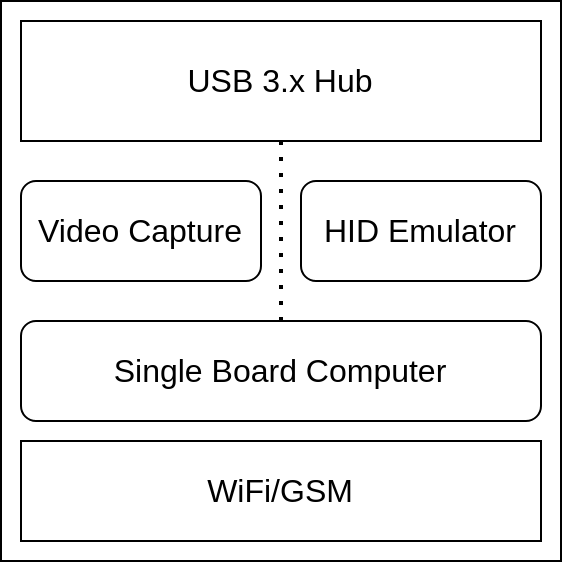
\includegraphics[width=0.56\linewidth]{./Figs/attack_model.png}
	\caption{Attack Model}\shuqing{Need to be more compact.}
	\label{fig:attack_model}
\end{figure}
\textbf{Scripting Mode} This mode majorly relies on the ``HID Emulator'' to send constructed HID packet to the victim. These constructed HID packet will be interpreted by the victim as valid keystrokes and mouse moves. Thus the attacker can executes arbitrary scripts on the victim's device. This is the function of the original BadUSB. Based on this, we made the following improvement.

First \tool supports defense mechanism bypass. As the original BadUSB cannot get feedback from the victim, defense mechanism like GoodUSB \cite{tian2015defending} is sufficient to prevent these BadUSB attack. But such defense mechanism needs visual notification to request authorization for unknown USB device. This means that when the defense request authorization from the user, our \tool is able to capture the content of authorization challenge and complete it. After the defense is bypassed, \tool continues the emulation and script execution, resulting a successful attack.

Moreover, as the mouse relies on the visual feedback to work properly, its emulation and automation were not supported by the original version of BadUSB. Yet with the video output support from USB 3.x, our \tool implements full-functional mouse emulation. This function enables attacks toward pure GUI programs and showed great potential in mobile attack scenario. Details can be obtained in Section~\ref{sec:experiment}.

The advantage of this mode is that it archives defense bypass and attack feedback with low overhead. As mentioned above, we only require video stream at the begin(defense bypass) and the end(result feedback) of the attack. Moreover, with mouse supported, \tool extends the original BadUSB attack surface and perform well in mobile device.

\textbf{Privacy Extraction Mode}
\tool under this mode does not emulate other USB device and solely relies on the video stream function of USB 3.x and use ``Video Capture'' component to transmit the stream to the embedded computer. The victim's device will mistakenly treat \tool as a external monitor and try to output its video stream. This stream is latter processed by the embedded computer to extract private data.

When running in this mode, \tool passively process the victim's video stream and detect for ``valuable'' private data.  Here, a data is ``valuable'' or not is decided by a customized detector, we implement a simple payment code detector for demonstration purpose. Though this detector is simple to implement, we successfully transfer money from the victim. More detail can be obtained in Section~\ref{sec:experiment}.

It is worth mentioning that \tool under this mode is completely passive, making it hard to be detected and defended. With different detector implemented, \tool under this mode is capable of serving more purpose.

\textbf{Remote Control Mode}
In \tool, we have implemented all components required to control a computer/mobile remotely, including a video stream and a keyboard/mouse emulation. Thus with all components enabled, not only will the victim's device treat \tool as a external display, but also a valid HID input source. Hence we can archive complete hijack of victim's device.

\tool under this mode follows a simple logic. \tool will receive video stream from the victim's device and redirect it to the attacker via GSM/WiFi. In the meanwhile, \tool also receives keystrokes and mouse movement from the attacker through GSM/WiFi and replay them to the victim by USB emulation.

This mode enable attacker to perform delicate operation that is beyond automation. Moreover, this mode provides a backdoor that does not require host network and thus is undetectable by the firewall running on the host machine.
\hongyi{I think this is a quite good selling point?}\shuqing{Agree with Hongyi.}

The advantage of this mode is that it can completely hijack the victim device and provide a backdoor beyond detection of firewalls. But this complete control also comes with the price of high power consumption and risk of being detected by the user.

